\chapter{Tutorial Sending Data (Java)}

\section{Scope}

This tutorial shows how data will be sent in a eTrice model. Within the example you will create two actors (MrPing and MrPong). MrPong will simply loop back every data it received.
MrPing will send data and verify the result.   

You will perform the following steps:

\begin{enumerate}
\item create a new model from scratch
\item create a data class
\item define a protocol with attached data
\item create an actor structure
\item create two simple state machines
\item build and run the model
\end{enumerate}

\section{Create a new model from scratch}

Remember exercise \textit{HelloWorld}.
Create a new eTrice project and name it \textit{SendingData}.
Open the \textit{SendingData.room} file and copy the following code into the file or use content assist to create the model.


\begin{verbatim} 
RoomModel SendingData {
    LogicalSystem SendingData_LogSystem {
        SubSystemRef SendingDataAppl:SendingData_SubSystem 
    }
    SubSystemClass SendingData_SubSystem {
        ActorRef SendigDataTopRef:SendingDataTop 
    }
    ActorClass SendingDataTop {
    }
}
\end{verbatim}

\section{Add a data class}

Position the cursor outside any class definition and right click the mouse within the editor window. From the context menu select \textit{Content Assist} (or Ctrl+Space).  

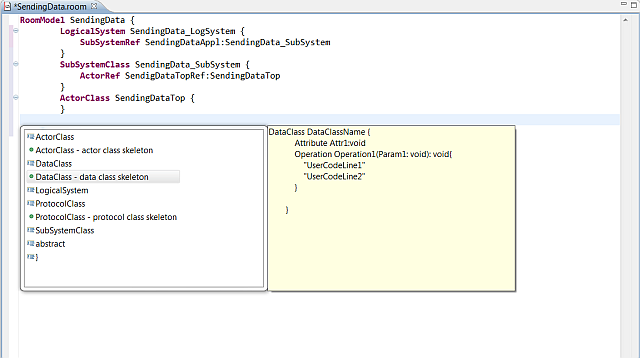
\includegraphics[width=\linewidth]{images/025-SendingData01.png}
% !images/025-SendingData01.png!

Select \textit{DataClass - data class skeleton} and name it \textit{DemoData}.
Remove the operations and add the following Attributes:

\begin{verbatim}
DataClass DemoData {
    Attribute int32Val: int32 = "4711"
    Attribute int8Array [ 10 ]: int8 = "{1,2,3,4,5,6,7,8,9,10}"
    Attribute float64Val: float64 = "0.0"
    Attribute stringVal: string = "\"empty\""
}
\end{verbatim}

Save the model and visit the outline view.
Note that the outline view contains all data elements as defined in the model. 

\section{Create a new protocol}

With the help of \textit{Content Assist} create a \textit{ProtocolClass} and name it \textit{PingPongProtocol}. Create the following messages:

\begin{verbatim} 
ProtocolClass PingPongProtocol {
    incoming {
        Message ping(data: DemoData)
        Message pingSimple(data:int32)
    }
    outgoing {
        Message pong(data: DemoData)
        Message pongSimple(data:int32)
    }
}    
\end{verbatim}

\section{Create MrPing and MrPong Actors}

With the help of \textit{Content Assist} create two new actor classes and name them \textit{MrPing} and \textit{MrPong}. The resulting model should look like this:

\begin{verbatim}
RoomModel SendingData {

    LogicalSystem SendingData_LogSystem {
        SubSystemRef SendingDataAppl: SendingData_SubSystem
    }

    SubSystemClass SendingData_SubSystem {
        ActorRef SendigDataTopRef: SendingDataTop
    }

    ActorClass SendingDataTop { }

    DataClass DemoData {
        Attribute int32Val: int32 = "4711"
        Attribute int8Array [ 10 ]: int8 = "{1,2,3,4,5,6,7,8,9,10}"
        Attribute float64Val: float64 = "0.0"
        Attribute stringVal: string = "\"empty\""
    }

    ProtocolClass PingPongProtocol {
        incoming {
            Message ping(data: DemoData)
            Message pingSimple(data: int32)
        }
        outgoing {
            Message pong(data: DemoData)
            Message pongSimple(data: int32)
        }
    }

    ActorClass MrPing {
        Interface { }
        Structure { }
        Behavior { }
    }

    ActorClass MrPong {
        Interface { }
        Structure { }
        Behavior { }
    }
} 

\end{verbatim}

The outline view should look like this:

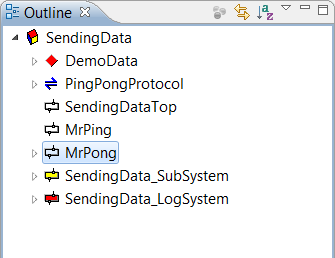
\includegraphics{images/025-SendingData03.png}
% !images/025-SendingData03.png!

\section{Define Actor Structure and Behavior}

Save the model and visit the outline view. Within the outline view, right click on the \textit{MrPong} actor and select \textit{Edit Structure}. Select an \textit{Interface Port} from the toolbox and add it to MrPong. Name the Port \textit{PingPongPort} and select the \textit{PingPongProtocol}.

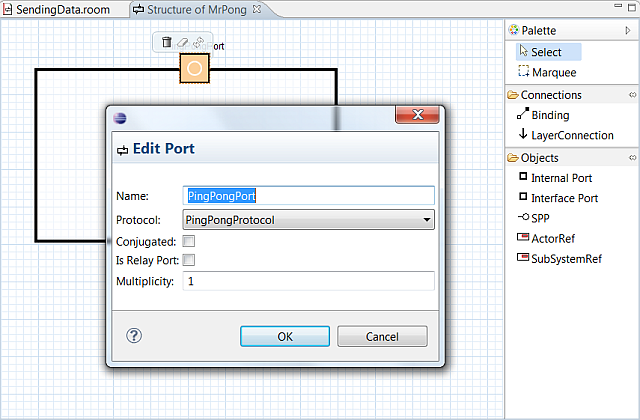
\includegraphics[width=\linewidth]{images/025-SendingData02.png}
% !images/025-SendingData02.png!

Do the same with MrPing but mark the port as \textit{conjugated}

\subsection{Define MrPongs behavior}

Within the outline view, right click MrPong and select \textit{Edit Behavior}. Create the following state machine:

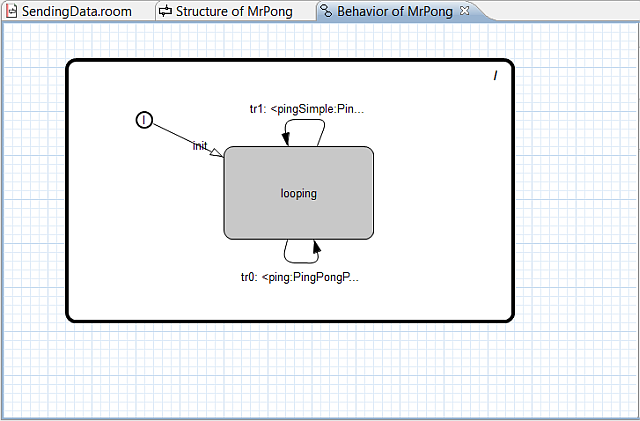
\includegraphics[width=\linewidth]{images/025-SendingData04.png}
% !images/025-SendingData04.png!

The transition dialogues should look like this:
For \textit{ping}:

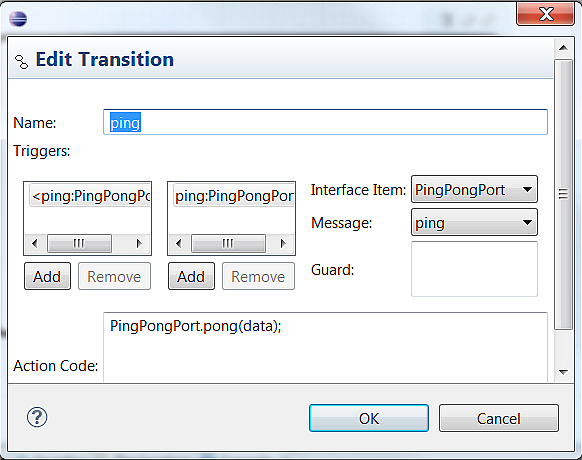
\includegraphics[width=\linewidth]{images/025-SendingData05.png}
% !images/025-SendingData05.png!

For \textit{pingSimple}:

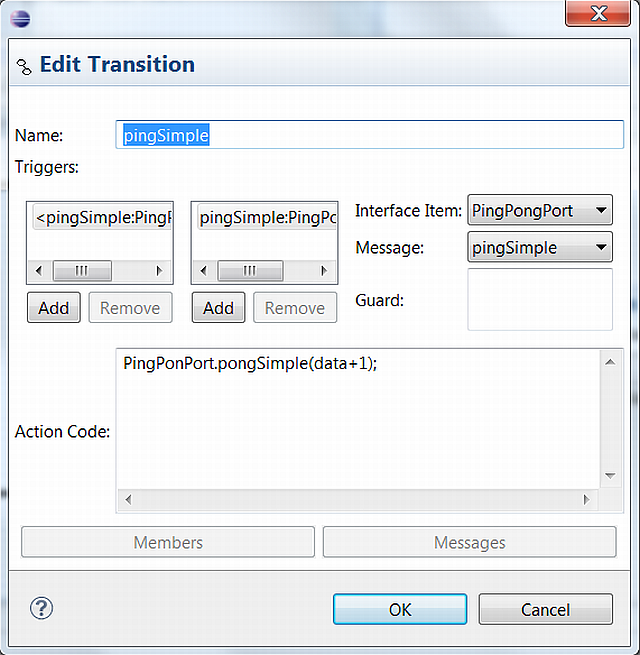
\includegraphics[width=\linewidth]{images/025-SendingData06.png}
% !images/025-SendingData06.png!


\subsection{Define MrPing behavior}

Within the outline view double click MrPing. Navigate the cursor to the behavior of MrPing. With the help of content assist create a new operation.

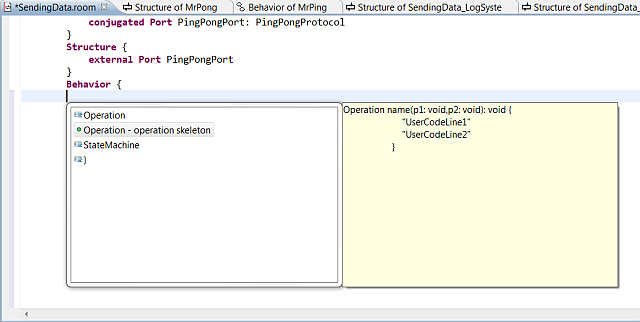
\includegraphics[width=\linewidth]{images/025-SendingData07.png}
% !images/025-SendingData07.png!

Name the operation \textit{printData} and define the DemoData as a parameter.

Fill in the following code:

\begin{small}
\begin{verbatim}
Operation printData(d: DemoData) : void {
            "System.out.printf(\"d.int32Val: %d\\n\",d.int32Val);"
            "System.out.printf(\"d.float64Val: %f\\n\",d.float64Val);"
            "System.out.printf(\"d.int8Array: \");"
            "for(int i = 0; i<d.int8Array.length; i++) {"
            "System.out.printf(\"%d \",d.int8Array[i]);}"
            "System.out.printf(\"\\nd.stringVal: %s\\n\",d.stringVal);"
}
\end{verbatim}
\end{small}

For MrPing create the following state machine:
(Remember that you can copy and paste the action code from the tutorial directory.)

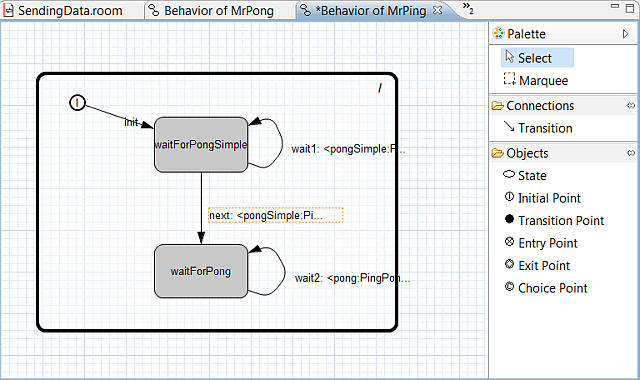
\includegraphics[width=\linewidth]{images/025-SendingData08.png}
% !images/025-SendingData08.png!

The transition dialogues should look like this:

For \textit{init}:

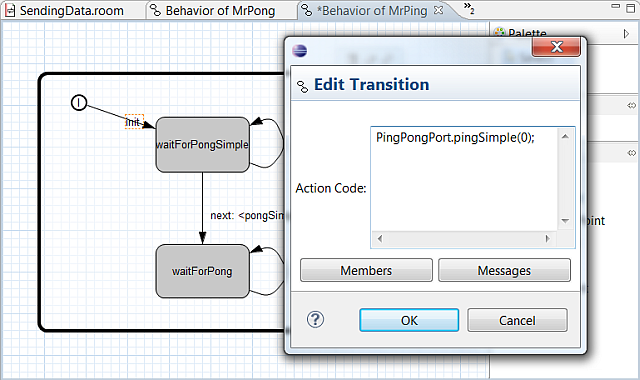
\includegraphics[width=\linewidth]{images/025-SendingData09.png}
% !images/025-SendingData09.png!

For \textit{wait1}:

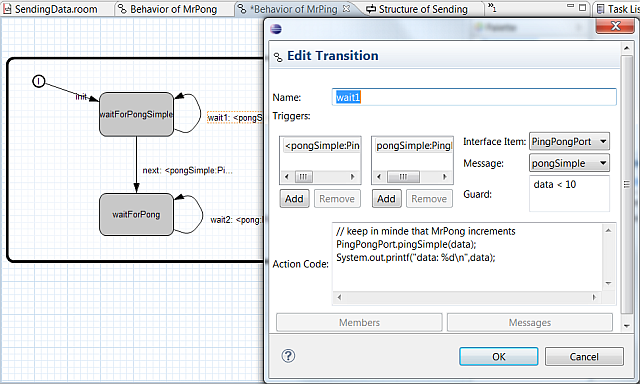
\includegraphics[width=\linewidth]{images/025-SendingData10.png}
% !images/025-SendingData10.png!

For \textit{next}:

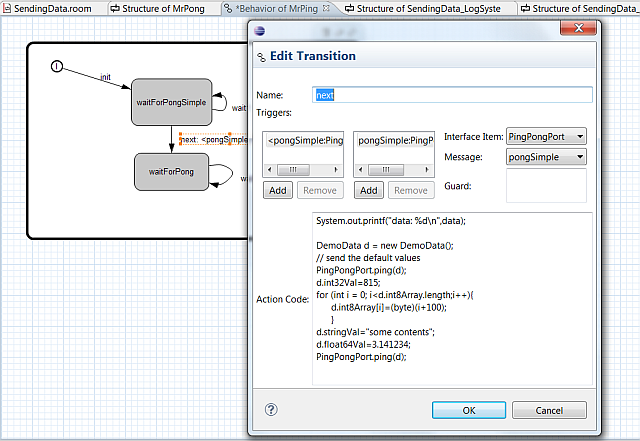
\includegraphics[width=\linewidth]{images/025-SendingData11.png}
% !images/025-SendingData11.png!

For \textit{wait2}:

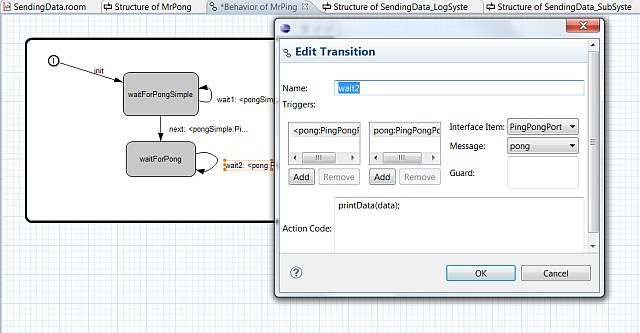
\includegraphics[width=\linewidth]{images/025-SendingData12.png}
% !images/025-SendingData12.png!

\section{Define the top level}

Open the Structure from SendingDataTop and add MrPing and MrPong as a reference. Connect the ports.

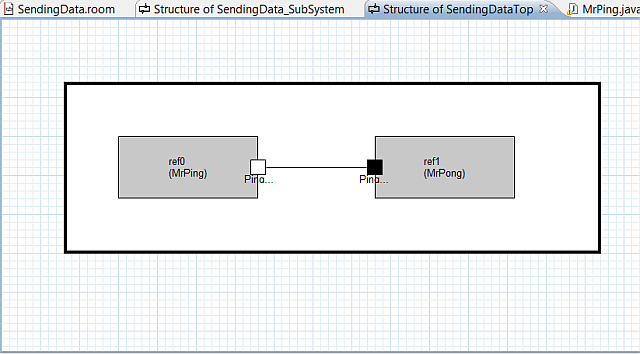
\includegraphics[width=\linewidth]{images/025-SendingData13.png}
% !images/025-SendingData13.png!

\begin{flushleft}The model is finished now and can be found in /org.eclipse.etrice.tutorials/model/SendingData.\end{flushleft}

\section{Generate and run the model}

Generate the code by right click to \textbf{gen\_SendingData.launch} and run it as \textbf{gen\_SendingData}. Run the model. 
The output should look like this:

\begin{verbatim}
type 'quit' to exit
/SendingData_SubSystem/SendigDataTopRef/ref0 -> waitForPongSimple
/SendingData_SubSystem/SendigDataTopRef/ref1 -> looping
/SendingData_SubSystem/SendigDataTopRef/ref1 -> looping
data: 1
/SendingData_SubSystem/SendigDataTopRef/ref0 -> waitForPongSimple
/SendingData_SubSystem/SendigDataTopRef/ref1 -> looping
data: 2
/SendingData_SubSystem/SendigDataTopRef/ref0 -> waitForPongSimple
/SendingData_SubSystem/SendigDataTopRef/ref1 -> looping
data: 3
/SendingData_SubSystem/SendigDataTopRef/ref0 -> waitForPongSimple
/SendingData_SubSystem/SendigDataTopRef/ref1 -> looping
data: 4
/SendingData_SubSystem/SendigDataTopRef/ref0 -> waitForPongSimple
/SendingData_SubSystem/SendigDataTopRef/ref1 -> looping
data: 5
/SendingData_SubSystem/SendigDataTopRef/ref0 -> waitForPongSimple
/SendingData_SubSystem/SendigDataTopRef/ref1 -> looping
data: 6
/SendingData_SubSystem/SendigDataTopRef/ref0 -> waitForPongSimple
/SendingData_SubSystem/SendigDataTopRef/ref1 -> looping
data: 7
/SendingData_SubSystem/SendigDataTopRef/ref0 -> waitForPongSimple
/SendingData_SubSystem/SendigDataTopRef/ref1 -> looping
data: 8
/SendingData_SubSystem/SendigDataTopRef/ref0 -> waitForPongSimple
/SendingData_SubSystem/SendigDataTopRef/ref1 -> looping
data: 9
/SendingData_SubSystem/SendigDataTopRef/ref0 -> waitForPongSimple
/SendingData_SubSystem/SendigDataTopRef/ref1 -> looping
data: 10
/SendingData_SubSystem/SendigDataTopRef/ref0 -> waitForPong
/SendingData_SubSystem/SendigDataTopRef/ref1 -> looping
/SendingData_SubSystem/SendigDataTopRef/ref1 -> looping
d.int32Val: 4711
d.float64Val: 0,000000
d.int8Array: 1 2 3 4 5 6 7 8 9 10 
d.stringVal: empty
/SendingData_SubSystem/SendigDataTopRef/ref0 -> waitForPong
d.int32Val: 815
d.float64Val: 3,141234
d.int8Array: 100 101 102 103 104 105 106 107 108 109 
d.stringVal: some contents
/SendingData_SubSystem/SendigDataTopRef/ref0 -> waitForPong
quit
echo: quit
\end{verbatim}

\section{Summary}

Within the first loop an integer value will be incremented by \textit{MrPong} and sent back to \textit{MrPing}. As long as the guard is true \textit{MrPing} sends back the value.

Within the \textit{next} transition, \textit{MrPing} creates a data class and sends the default values. Then \textit{MrPing} changes the values and sends the class again. At this point you should note that during the send operation, a copy of the data class will be created and sent. Otherwise it would not be possible to send the same object two times, even more it would not be possible to send a stack object at all. This type of data passing is called \textit{sending data by value}.
However, for performance reasons some applications requires \textit{sending data by reference}. In this case the user is responsible for the life cycle of the object. In Java the VM takes care of the life cycle of an object. This is not the case for C/C++. Consider that a object which is created within a transition of a state machine will be destroyed when the transition is finished. The receiving FSM would receive an invalid reference. Therefore care must be taken when sending references.      

For sending data by reference you simply have to add the keyword \textit{ref} to the protocol definition.
 
\begin{verbatim}Message ping(data: DemoData ref)\end{verbatim}

Make the test and inspect the console output.
